\chapter{Revisão Bibliográfica}\label{chap:revisao}

\section{Considerações Iniciais}

% A literatura em redução de dimensionalidade é extensa e os métodos desenvolvidos apresentam grande diversidade em relação a aspectos matemáticos e computacionais. Buscando uma melhor contextualização, esta seção aborda apenas trabalhos que buscam de alguma forma utilizar representações visuais para a execução desta tarefa.

Os trabalhos do atual estado da arte que mais se assemelham ao o aqui proposto aparecem sobre o nome de métodos de redução de dimensionalidade. 
A redução de dimensionalidade é o processo realizado para se representar dados de alta dimensionalidade em um espaço de menor dimensionalidade, onde, idealmente, o espaço reduzido corresponde à dimensionalidade intrínseca dos dados. 
Por sua vez, a dimensionalidade intrínseca dos dados é o conjunto mínimo de variáveis necessário para descrever as propriedades dos dados~\cite{Fukunaga1990}.

Dentre os propósitos da redução de dimensionalidade, os principais são a melhoria na eficiência dos métodos que operam sobre os dados e a redução do custo computacional desses métodos.  
\citeauthor{Konig2000}~\cite{Konig2000}, por exemplo, apresenta melhorias na precisão de sistemas de classificação e no desempenho de sistemas de reconhecimento automático ao preceder os procedimentos com o processo de redução de dimensionalidade. 
Até mesmo outros benefícios não tão diretos podem ser alcançados por meio do uso de técnicas de redução. 
Trata-se do caso do mesmo trabalho apresentado por \citeauthor{Konig2000}, onde métodos de redução de dimensionalidade são utilizados para reduzir a complexidade de designs de circuitos integrados, resultando em uma redução na área e no consumo de energia dos circuitos.

Uma terceira utilidade para os métodos de redução de dimensionalidade é viabilizar a construção de representações visuais de dados multidimensionais~\footnote{No contexto de visualização computacional, conjuntos de dados multidimensionais são aqueles com mais do que três atributos.}, permitindo que sejam mapeados em um espaço bidimensional (tela computador).
Representações visuais dos dados são cruciais para a análise exploratória de dados, principalmente para investigações iniciais dos dados, onde ainda não se conhece as propriedades dos dados~\cite{Kaski2011}. 

A literatura em redução de dimensionalidade é extensa e os métodos desenvolvidos apresentam grande diversidade em relação a aspectos matemáticos e computacionais. 
Buscando uma melhor organização, este capítulo foi dividido em duas seções. 
A primeira busca descrever sucintamente os métodos automáticos e apresentar suas limitações, principalmente evidenciar que a falta da participação do usuário no processo faz com que muitas vezes os resultados obtidos não sejam facilmente compreendidos. 
A segunda seção apresenta os métodos que permitem que o usuário participe do processo de redução de dimensionalidade por meio da interação com representações visuais. 
Ao longo da segunda seção discute-se que apesar dos métodos interativos se mostrarem como uma interessante alternativa, os mecanismos de interação propostos apresentam grandes limitações. 
Nas considerações finais deste capítulo, resume-se as principais limitações dos métodos interativos. 

\section{Redução de Dimensionalidade Automática}

A redução de dimensionalidade automática pode ser realizada seguindo duas abordagens. 
A primeira transforma os atributos de entrada em um novo conjunto de dimensões que busca conservar certas propriedades ou relacionamentos do conjunto original. 
Por extrair um novo conjunto de atributos a partir dos dados originais, esta abordagem recebe o nome de extração de características (\emph{feature extraction}).
Já a segunda abordagem busca selecionar quais dos atributos do conjunto de dados são realmente relevantes para a análise segundo algum critério. 
Como os dados não são modificados, esta segunda abordagem é chamada de seleção de características (\emph{feature selection}).

\subsection{Extração de Características}

O problema de extração de características pode ser descrito da seguinte forma: 
Dado um conjunto de dados representado por uma matriz $\textbf{X}$ composta por $n$ vetores $\textbf{x}_i~(i \in \{1,2,...,n\})$ $m-$dimensionais, deseja-se encontrar uma transformação $t: \textbf{X} \rightarrow \textbf{Y}$, onde $\textbf{Y}$ trata-se de uma matriz composta por $n$ vetores $\textbf{y}_i~(i \in \{1,2,...n\}$ de dimensionalidade $p$ ($p < m$). 
Normalmente $p \ll m$ e, idealmente, $p$ equivale à dimensionalidade intrínseca dos dados, fazendo com que $t$ mantenha em $\textbf{Y}$ o máximo das propriedades de $\textbf{X}$ quanto for possível. 

Como apresentado por~\citeauthor{Maaten2009}~\cite{Maaten2009}, existe uma grande variedade de métodos de extração de características. Não é intuito desta subseção detalhar cada uma dessas técnicas e levantar suas limitações particulares, mas sim ilustrar a limitação que todas apresentam em comum de retornar resultados pouco intuitivos para o usuário e impedi-lo de interagir com os dados. Para este fim, o método de análise de componentes principais (PCA) será utilizado como base para os exemplos.

Popular dimension reduction approaches, such as Principal Component Analysis [Jolliffe 1986], Multidimensional Scaling [Mead 1992], and Kohonen’s Self Organizing Maps [Kohonen1995; Flexer 1999], condense the hundreds or thousands of dimensions into a few dimensions. However, those generated dimensions have little intuitive meaning to users and allow little user interaction.

% LER OS PAPERS DE RED DIM PARA INSPIRAÇÃO E REFERÊNCIAS.

% Existem três principais abordagens para se reduzir a dimensionalidade dos conjuntos de dados a partir da combinação dos atributos. Análise de Componentes Principais (\textit{Principal Component Analysis)}~ ou simplesmente PCA, realiza combinações lineares sobre os atributos de modo que o novo espaço agregue a maior parte da variância dos dados. Para análises onde relações não lineares devem ser consideradas, \textit{Multimensional Scaling} (MDS) é uma alternativa interessante, pois trata-se de um algoritmo de otimização iterativo não linear, que busca minimizar as distâncias entre os elementos no espaço projetado e no espaço original. A área de aprendizado de máquina contribuiu com o método não supervisionado \textit{Self Organizing Maps} (SOM) para transformar conjuntos de dados em mapas bidimensionais.

% Sem dúvida a técnica mais importante é PAC

\subsection{Seleção de Características} 

O objetivo dos métodos de seleção de características é encontrar o subconjunto  dos atributos de entrada mais adequado para a aplicação em estudo. 
Assim, busca-se identificar e eliminar atributos redundantes~\cite{Kohavi1997} ou que não apresentem correlação com o fenómeno investigado~\cite{Nilsson2007}. 
Por exemplo, em tarefas de classificação supervisionada, pode-se determinar a importância de um atributo avaliando sua correlação com o atributo classe. Os métodos de seleção dividem-se basicamente em filtros, \emph{wrappers} e métodos incorporados~\cite{Guyon2003}. 

Filtros utilizam um atributo alvo como referência e determinam, por meio de alguma medida de correlação, quanto cada atributo se relaciona com esta referência. 
A filtragem é realizada descartando os atributos que apresentam relação menor do que um valor fixado.
Uma das desvantagens de filtros é que pelo fato de considerarem somente relações para par, não são capazes de detectar dependências indiretas entre os atributos. 

O funcionamento de \emph{wrappers} e métodos embutidos consiste em realizar uma busca sobre subconjuntos candidatos e tomar como resultado o subconjunto que resulta na melhor precisão de um algoritmo de predição.
O caso completo trata-se da avaliação de $2^m$ subconjuntos, onde $m$ corresponde ao número de atributos do conjunto de entrada. 
Tal situação equivale a um problema $np$-completo~\cite{Amaldi1998}, consequentemente para grandes conjuntos de dados a solução ótima não pode ser obtida em tempo fazível, exigindo assim a adoção de alguma eurística. 
A distinção entre os dois métodos vem de que \emph{wrappers} enxergam o método de predição como uma caixa-preta, se interessando somente pelo resultado obtido, permitindo que diferentes preditores sejam aplicados sem a necessidade de modificar o método de seleção. Já os métodos embutidos, como o nome sugere, são incorporados às etapas de treinamento dos preditores, sendo assim específicos para cada situação. 

Em comparação aos métodos de extração, os métodos de seleção apresentam a vantagem de que o resultado obtido é mais intuitivo ao usuário, pois se trata de um subconjunto dos atributos de entrada. 
Assim, se o usuário tem certo conhecimento sobre o conjunto de entrada, então será capaz de compreender os resultados obtidos.
No entanto, eles compartilham a mesma natureza caixa-preta dos métodos de extração e privam o usuário de qualquer interação durante o processo de redução, impedindo que o usuário contribua com seu conhecimento sobre o domínio e compreenda quais características dos seus dados foram responsáveis por aquele resultado.

\section{Redução de Dimensionalidade Interativa}

Métodos visuais que permitem a interação do usuário ganharam grande popularidade nos últimos anos~\cite{State2012}. 
Grande parte deste sucesso pode ser atribuído ao uso efetivo da capacidade preemptiva da visão humana.
Foi demonstrado que quando os dados são representados por alguma forma gráfica, o ser humano é capaz de detectar e reconhecer padrões facilmente e rapidamente~\cite{Healey1995}, mesmo em grandes conjuntos de dados~\cite{Fodor2002}.
Mas a capacidade preemptiva de visão humana não é a única vantagem dos métodos interativos. Permitir que o usuário participe ativamente nos processos e na geração dos resultados também traz grandes benefícios em relação a métodos completamente automáticos.
Deste modo, a seguir serão apresentados os trabalhos desta nova vertente que buscam executar redução de dimensionalidade de forma interativa. Trabalhos que não somente fazem uso da capacidade perceptiva dos usuários, mas que também permitem que o usuário participe ativamente na geração dos resultados com o seu conhecimento sobre o domínio.

\subsection{Hierarquias de Dimensões}

Em busca de construir espaços de baixa dimensionalidade mais intuitivamente do que pelo uso de métodos automáticos, \citeauthor{Yang2003} desenvolveram o método de redução de dimensionalidade chamado VHDR (Visual Hierarchical Dimensions Reduction)~\cite{Yang2003}. O funcionamento deste método é ilustrado pela Figura~\ref{fig:vhdr1}. Inicialmente constrói-se uma organização hierárquica dos atributos com base na similaridade entre as dimensões. Em seguida, com base nesta hierarquia, o usuário define grupos de dimensões. Finalmente, o usuário por meio de um método automático ou de seu conhecimento sobre os dados, escolhe dimensões representativas para cada grupo, reduzindo assim a dimensionalidade dos dados. 

\begin{figure}[h!]
  \centering
  \begin{subfigure}[b]{0.4\textwidth}
    \centering
    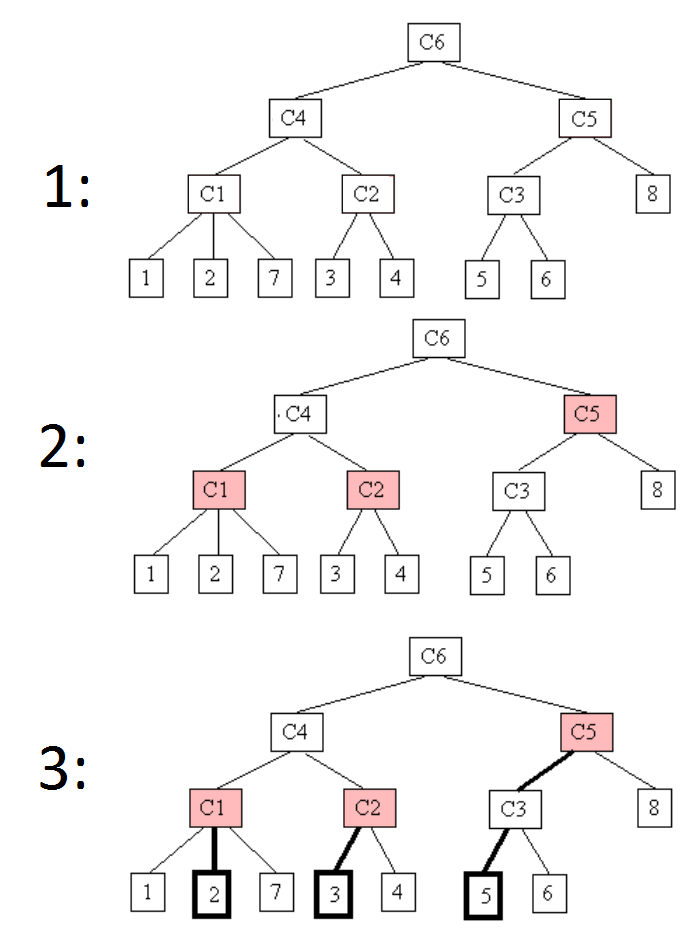
\includegraphics[width=\textwidth]{images/vhdr1.png}
    \caption{}
    \label{fig:vhdr1}
  \end{subfigure}%
  \qquad %add desired spacing between images, e. g. ~, \quad, \qquad etc.
  \begin{subfigure}[b]{0.45\textwidth}
    \centering
    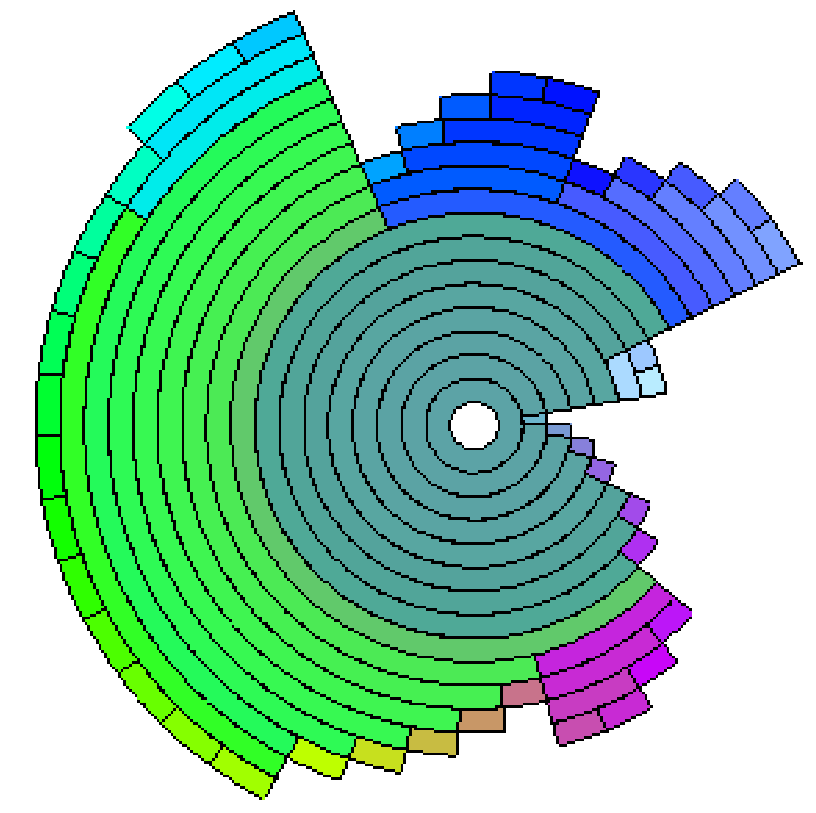
\includegraphics[width=\textwidth]{images/vhdr2.png}
    \caption{}
    \label{fig:vhdr2}
  \end{subfigure}
  \caption[VHDR: Visual Hierarchical Dimension Reduction]{(a) Ilustração do funcionamento do VHDR. Inicialmente (1), constrói-se uma organização hierárquica dos atributos. Em seguida (2), o usuário define grupos de dimensões com base na escolha de níveis de cortes da árvore. Finalmente (3), o usuário por meio de um método automático ou de seu conhecimento sobre os dados, escolhe dimensões representativas para cada grupo, reduzindo assim a dimensionalidade dos dados. (b) Exemplo da representação gráfica InterRing para um conjunto com 42 dimensões e $20.000$ elementos. O nó raiz da árvore é representado pelo círculo mais interno e os nós folhas pelos elementos posicionados na borda. As cores são utilizadas para destacar grupos de dimensões com características em comum.}
\end{figure}

O processo de construção da hierarquia é muito semelhante aos algoritmos de agrupamento hierárquico. A distinção é que agrupa-se atributos semelhantes, ao invés de itens. Deste modo, qualquer método de agrupamento pode ser aplicado, exigindo-se apenas que o agrupamento resulte em uma estrutura hierárquica, no caso uma árvore, onde cada dimensão seja representada por um nó folha da árvore. 

Uma limitação do VHDR surge quando se inicia a etapa de seleção de dimensões representativas. A representação visual não é capaz de transmitir a magnitude da similaridade entre os atributos. Isto é, o usuário não é capaz de compreender, por exemplo, quanto um elemento dentro de um grupo é diferente de outro elemento pertencente a outro grupo. Essa limitação dificulta tanto a etapa de seleção de grupos quanto a de escolha de dimensões representativas.

Os autores do VHDR desenvolveram uma extensão chamada DOSFA (Dimension Ordering Spacing and Filtering Approach)~\cite{DOSFA} que apresenta outros mecanismos para manipular os atributos de um conjunto de dados. Mais especificamente, eles propõem três abordagens para ordenação, espaçamento e filtragem de atributos. As duas primeiras, ordenação e espaçamento, não estão diretamente relacionadas com redução de dimensionalidade. Já a filtragem de atributos é análoga aos métodos de seleção de características. Este mecanismo consiste em remover dimensões pouco representativas ou redundantes. De modo que se certas dimensões apresentam alta similaridade entre si, então apenas uma delas é mantida. Ou se certas dimensões apresentam pouca relevância, então são descartadas. A grande complexidade do processo de filtragem é o modo como se define a redundância e a importância entre as dimensões. 

Tanto o VHDR quanto o DOSFA tratam todo o conjunto de dados de maneira uniforme. No entanto, podem existir subconjuntos nos dados com diferentes características que devem ser analisados separadamente~\cite{May2011}. Uma maneira de contornar este problema seria apresentar os itens simultaneamente com a representação das dimensões, assim o usuário poderia detectar grupos não somente nas dimensões mais também nos itens.

\subsection{Mapeamento de Dimensões no Plano}

Abordando justamente o problema de se apresentar itens simultaneamente com as dimensões de um conjunto de dados, \citeauthor{Yang2004} desenvolveram a técnica VaR (Value and Relation)~\cite{Yang2004}. A técnica une os conceitos de MDS e glifos para representar as dependências entre as dimensões de uma base de dados. 

Como mostra a Figura~\ref{fig:var1}, cada glifo representa uma dimensão e de acordo com seus posicionamentos no plano o usuário pode compreender como as dimensões se relacionam entre si. 
O usuário é capaz de construir espaços dimensionais reduzidos que conservam certas características dos dados por meio de seleções sobre os dados ou pelo uso de um método automático que a partir de uma dimensão de referência e um \emph{threshold} definido pelo usuário retorna as dimensões mais semelhantes.

\begin{figure}[h!]
  \centering
  \begin{subfigure}[b]{0.5\textwidth}
    \centering
    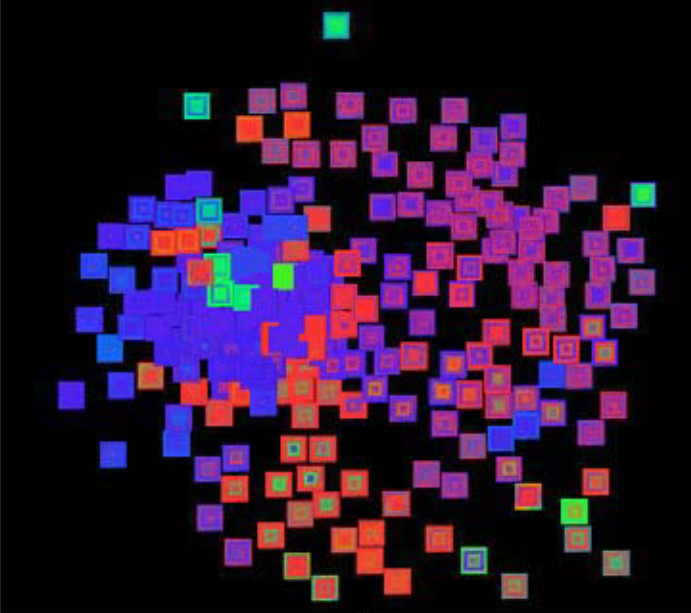
\includegraphics[width=\textwidth]{images/var1.png}
    \caption{}
    \label{fig:var1}
  \end{subfigure}%
  ~ %add desired spacing between images, e. g. ~, \quad, \qquad etc.
  \begin{subfigure}[b]{0.475\textwidth}
    \centering
    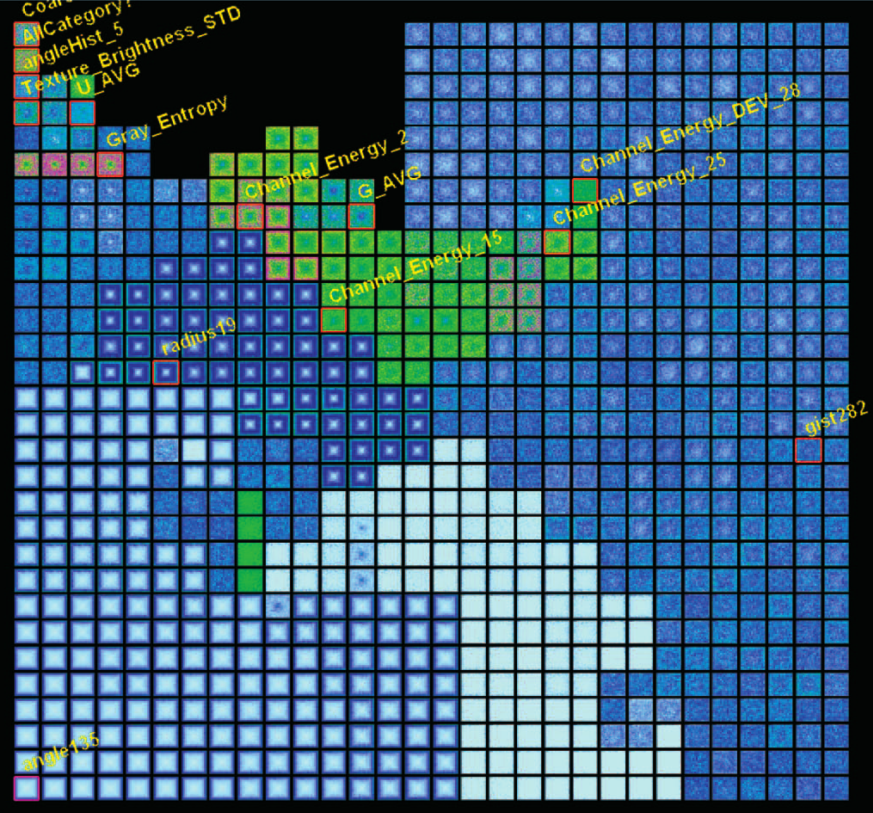
\includegraphics[width=\textwidth]{images/var2.png}
    \caption{}
    \label{fig:var2}
  \end{subfigure}
  \caption[VaR: Value and Relation]{(a) Exemplo da técnica VaR para um conjunto de $50.000$ itens e $361$ dimensões. Cada dimensão é representada por um glifo e seus posicionamentos refletem a similaridade entre as dimensões, de modo que glifos que se encontram próximos indicam atributos que apresentam alguma relação entre si. É possível notar certas sobreposições entre os glifos, condição que pode dificultar as análises realizadas pelo usuário. (b) Exemplo de representação alternativa proposta como extensão da técnica VaR para um conjunto de 11.413 itens e 838 dimensões. O principal objetivo desta representação alternativa é evitar sobreposições de glifos ocorrente na versão anterior da técnica.}
\end{figure}

O procedimento para a construção desta visualização inicia pela construção de uma matriz de distâncias que é responsável por capturar os relacionamentos entre pares de dimensões do conjunto de dados. 
Sobre esta matriz de distâncias aplica-se uma técnica de MDS para mapear cada dimensão em uma posição do espaço bidimensional. 
Finalmente, cria-se um glifo orientado a pixels para cada dimensão que será utilizado para representar cada dimensão no plano.

Observando a Figura~\ref{fig:var1} é possível notar que o uso de glifos faz com que ocorram sobreposições, pois cada glifo requer um espaço relativamente grande para que seja observado adequadamente. 
As sobreposições dificultam as análises de regiões de interesse e podem fazer com que o usuário alcance conclusões inválidas, devido a oclusão de algum elemento importante. 
Buscando tratar este problema~\citeauthor{Yang2007} desenvolveram a extensão~\cite{Yang2007} ilustrada na Figura~\ref{fig:var2} para a técnica VaR, onde apresentaram alternativas para a projeção de glifos no plano. No entanto, por estabelecerem uma distância fixa entre os elementos, perde-se a informação de quanto duas dimensões são similares entre si. Assim, a alternativa proposta não é capaz de transmitir os relacionamentos entre as dimensões tão bem quanto o resultado obtido pela versão original.

Apesar do método VaR apresentar informações sobre itens e dimensões simultaneamente, não é permitido ao usuário interagir com os itens. Consequentemente, este método sofre das mesmas limitações dos métodos apresentados anteriormente, ou seja, não é capaz de tratar peculiaridades em subconjuntos dos dados. 
Um outro aspecto importante que os próprios autores mencionam em relação ao uso deste tipo de  glifos é que os usuários têm dificuldade em comparar glifos que se encontram afastados entre si. 

% Brushing: falar como continuidade de VaR

Não é especificamente um método para redução de dimensionalidade, mas serve como um exemplo de como apresentar itens e dimensões simultaneamente e permitir a interação do usuário em ambos sentidos.

A exploração das relações entre as dimensões não precisa estar vinculada somente a representações visuais dos atributos do conjunto de dados. \citeauthor{Turkay2011}~\cite{Turkay2011} propuseram um método de múltiplas visões que permite que o usuário interaja tanto com as dimensões quanto com os itens da base de dados. O principal mecanismo de interação é a seleção que se reflete em outras visões e permite que se visualize, por exemplo, as dimensões que melhor representam subconjuntos dos dados. Uma das limitações deste trabalho é falta de medidas que consideram pares de dimensões, como medidas de correlação, o que dificulta a observação de dependências entre os atributos.  

\subsection{Matrizes de Correlação}

Uma das maneiras mais utilizadas para se inspecionar relações entre dimensões são as matrizes de correlação~\cite{Friendly2002} (observar Figura~\ref{fig:var1}). Este tipo de representação é útil para se ter uma visão geral das relações entre pares de dimensões e permite que um grande número de itens seja analisado. No entanto, para análises mais detalhadas, ou que exijam uma comparação entre mais do que simplesmente pares de elementos, não é uma representação adequada.

\begin{figure}[h!]
    \centering
    \includegraphics[width=12cm]{images/bs1.pdf}
    \caption[Matrizes de Correlação]{Exemplo de matriz de correlação para dados de jogos de baseball. A cor azul indica correlação positiva entre as variáveis, enquanto a vermelha correlação negativa. A intensidade da cor é proporcional à magnitude da correlação. Com base em uma investigação visual é possível levantar certas hipóteses sobre os dados. Observa-se, por exemplo, uma relação direta entre os anos de carreira do jogador (Years) e o seu salário (logSal), ao mesmo tempo a experiência tem uma relação inversa com o número de erros.} 
    \label{fig:bs1}
\end{figure}

Devido à sua simplicidade, este tipo de representação foi adotada por diversos métodos visuais que viabilizam a investigação de atributos de um conjuntos de dados. O \emph{framework}\footnote{Explicar o que é framework} RBF (\emph{Rank by Feature})~\cite{RBF2004}, por exemplo, utiliza matrizes de correlação para apresentar um \emph{ranking} entre pares de dimensões (observar Figura~\ref{fig:rbf1}). Este \emph{ranking} é definido com base em critérios estatísticos estabelecidos pelo usuário. 

\begin{figure}[h!]
    \centering
    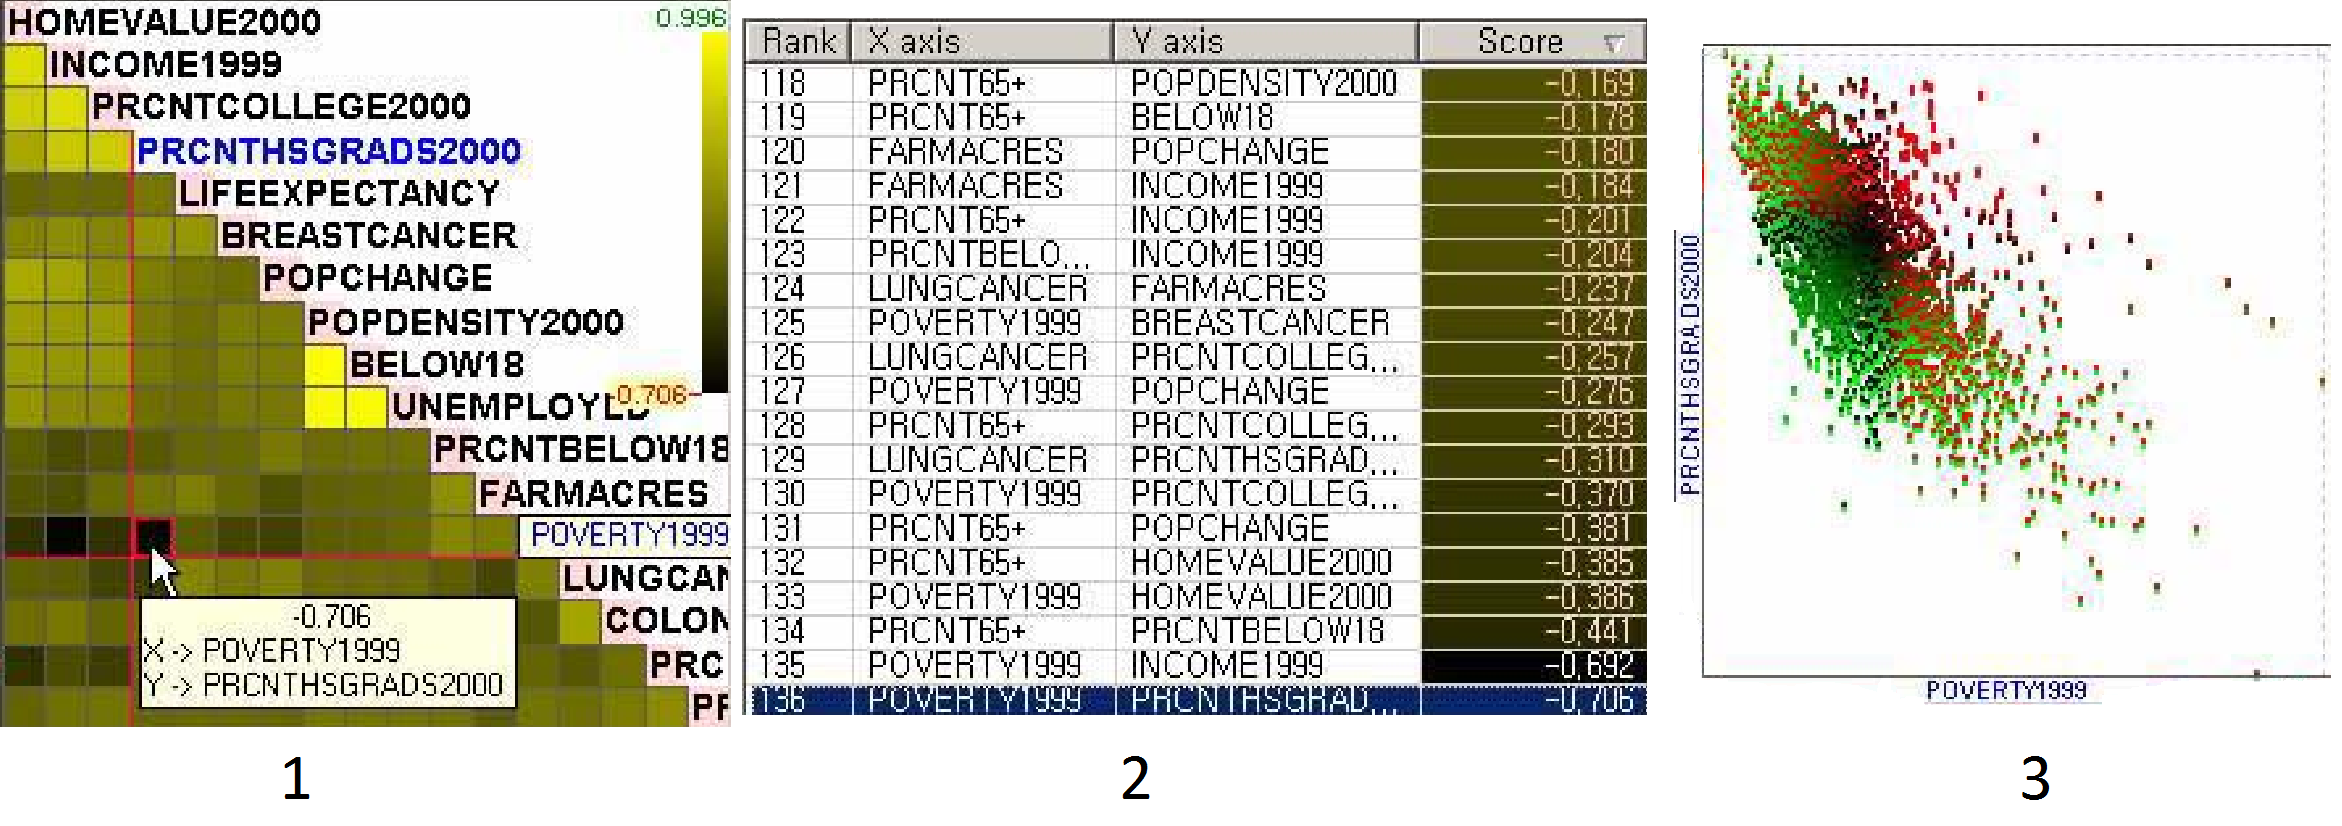
\includegraphics[width=\textwidth]{images/rbf1.png}
    \caption[Rank by Feature Framework]{Exemplo do \emph{framework Rank by Feature}. (1) matriz de correlação dos itens. (2) valores de correlação para os pares de dimensões. (3) projeção bidimensional das dimensões selecionadas \emph{(Extraído de \cite{RBF2004})}}.
    \label{fig:rbf1}
\end{figure}

O objetivo da investigação da matriz de correlação não é propriamente reduzir a dimensionalidade do conjunto de dados, mas sim encontrar subconjuntos de atributos com características similares. Outros trabalhos~\cite{Guo2003,MacEachren2003,May2011,May2011ss} adotam abordagens semelhantes ao do RBF para atingir este mesmo objetivo. Eles diferem na maneira de como é construída a matriz de correlação e de quais recursos são disponibilizados para o usuário interagir com os subconjuntos de dimensões.

Um problema geral desses trabalhos é que certas análises podem exigir demasiado esforço do usuário, devido à necessidade de se explorar individualmente cada dimensão ou avaliar par a par as relações entre atributos. Com a ocorrência de dependências não lineares este problema torna-se ainda maior e o usuário pode se perder em suas análises e não extrair novos conhecimentos dos resultados.

\subsection{Visualização de Métodos Automáticos}

Existem certos métodos que não utilizam a visualização para realizar redução em si, mas sim para tornar os métodos automáticos mais compreensivos. Eles buscam incluir a participação do usuário nesses métodos para tornar essas ``caixas pretas'' mais compreensivas. 

A técnica iPCA~\cite{Jeong2009}, por exemplo, provém meios para o usuário manipular os parâmetros da técnica PCA e, assim, ser capaz de entender mais facilmente as transformações realizadas sobre os dados. 

Similarmente, MDSteer [24] permite que o usuário guie o processo de MDS ao escolher regiões de interesse para se concentrar os esforços computacionais. No entanto, os mecanismos de interação propostos por esses trabalhos se baseiam em interfaces que são demasiadamente complexas ou que não contém todos os mecanismos necessários para lidar com um grande volume de dados.

\section{Considerações Finais}

A representação explícita das dimensões do conjunto de dados serve como inspiração para este trabalho de mestrado. Já o uso de glifos orientado a pixels se mostrou inadequado para situações com um elevado número de elementos, causando indesejadas sobreposições entre elementos. Um outro aspecto importante que os próprios autores mencionam em relação ao uso deste tipo de  glifos é que os usuários têm dificuldade em comparar glifos que se encontram afastados entre si. 

\begin{table}
    \centering
    \caption {legenda}
    \begin{tabular}{|c|C{2cm}|C{2cm}|C{2.5cm}|C{3cm}|}
        \hline
        \textbf{Técnica} & 
        \textbf{Interação com Itens} & 
        \textbf{Seleção de Atributos} &
        \textbf{Extração de Atributos} &
        \textbf{Transformação de Atributos}
        \\ \hline
        VHDR    & N & S & N & N \\
        DOSFA   & N & S & N & N \\
        VaR     & N & S & N & N \\
        \hline
    \end{tabular}
\end{table}

% Tendo em vista que o objetivo das representações visuais é tornar as análises mais intuitivas, qualquer tipo de obstáculo, como a necessidade de treinamento do usuário, pode ser desfavorável ao se comparar com os métodos automáticos.

% Métodos de coordenação tem sido muito utilizados, mas eles não se preocupam em manter a mesma metáfora visual.

% Carência de certos mecanismos de interação (nenhum propõe "arrastar dimensões", somente  selecionar e no máximo combiná-las) 
% Sobrecarga sistema cognitivo do usuário (density pixels, variedade de metáforas visuais)
